\documentclass[10pt,conference]{IEEEtran}

\usepackage[T1]{fontenc}
\usepackage{lmodern}
\usepackage{amsmath,amssymb}
\usepackage{graphicx}
\usepackage{booktabs}
\usepackage{array}
\newcolumntype{L}[1]{>{\raggedright\arraybackslash}p{#1}}
\usepackage{xcolor}
\usepackage{algorithm}
\usepackage{algpseudocode}
\usepackage{listings}
\usepackage{hyperref}
\usepackage{cite}
\usepackage{placeins}
\usepackage{balance}
\usepackage{microtype}

\graphicspath{{figures/}{diagrams/}}

\definecolor{ink}{HTML}{1A1A1A}
\definecolor{accent}{HTML}{A6192E}
\definecolor{codebg}{HTML}{F5F5F5}

\lstdefinestyle{go}{
  basicstyle=\ttfamily\scriptsize,
  breaklines=true,
  backgroundcolor=\color{codebg},
  frame=single,
  rulecolor=\color{black!25},
  framesep=3pt,
  columns=fullflexible,
  keywordstyle=\bfseries,
  commentstyle=\itshape\color{black!45},
  showstringspaces=false,
  xleftmargin=2pt, xrightmargin=2pt,
  aboveskip=6pt, belowskip=4pt,
}
\lstdefinestyle{sh}{
  basicstyle=\ttfamily\scriptsize,
  breaklines=true,
  backgroundcolor=\color{codebg},
  frame=single,
  rulecolor=\color{black!25},
  framesep=3pt,
  columns=fullflexible,
  showstringspaces=false,
  xleftmargin=2pt, xrightmargin=2pt,
  aboveskip=6pt, belowskip=4pt,
}

\hypersetup{
  colorlinks=true,
  linkcolor=accent!70!black,
  citecolor=accent!70!black,
  urlcolor=accent!70!black,
  pdftitle={otcat: The Netcat for Industrial I/O},
  pdfauthor={Moustafa Mahmoud Atta}
}

\newcommand{\otcat}{\texttt{otcat}}
\newcommand{\code}[1]{\texttt{#1}}

\title{\textbf{otcat}: The Netcat for Industrial I/O\\
\large A Minimalist, Verifiable Architecture for Register-Level Access to Operational Technology}

\author{
\IEEEauthorblockN{Moustafa Mahmoud Atta}
\IEEEauthorblockA{QuitOperation \\ v1.0.0 --- July 2026 \\
Email: MoustafaAt1a@outlook.com \\ GitHub: \url{https://github.com/MoustafaAt1a} \\
Project: \url{https://github.com/QuitOperation/otcat}}
}

\begin{document}
\maketitle

\begin{center}
\begin{minipage}{0.92\linewidth}
\centering
\itshape\small
``Software that speaks to physical machines should say only what it means,\\
refuse what it cannot verify, and never guess quietly.''
\normalfont\\[2pt]
\upshape\footnotesize --- the design motto of this work
\end{minipage}
\end{center}
\vspace{4pt}

\begin{abstract}
Reading a single register from a programmable logic controller (PLC)
today typically requires a vendor engineering suite, a configured OPC~UA
gateway, or a bespoke script wrapping a protocol library --- there is no
equivalent, for operational technology (OT), of what \code{netcat}
became for TCP/IP: a small, composable, stdin/stdout-native primitive
that any other tool can pipe into. This paper presents \otcat, a
zero-dependency command-line tool that streams typed register and coil
values from industrial devices to standard output and accepts written
values from standard input, following the Unix philosophy of doing one
thing well~\cite{mcilroy1978}. We give a complete, from-specification
implementation of Modbus TCP~\cite{modbus2012,modbus_tcp_guide}, formalize
its addressing ambiguities and multi-register codec as explicit,
tested transformations, and document a deliberate scope boundary: three
further protocols (EtherNet/IP, S7comm, BACnet/IP) are architecturally
wired into the tool's driver interface but not implemented, on the
grounds that an incorrect write path against a live controller is a
worse outcome than an honest ``not implemented'' error. We describe a
write-safety gate that treats every write as untrusted until explicitly
confirmed, a full-jitter exponential backoff strategy~\cite{brooker2015}
for long-running polling, and a verification methodology combining
property-based round-trip testing, coverage-guided fuzzing, and
integration testing against a physically-modeled control loop. We
report real, reproducible latency and throughput measurements and a
closed-loop demonstration in which \otcat\ observes a simulated
PI-controlled tank level end to end through an actual TCP socket. All
figures, benchmark numbers, and the demonstration trace in this paper
were produced by running the accompanying software; none are estimated.
\end{abstract}

\begin{IEEEkeywords}
industrial control systems, Modbus, operational technology, command-line
tools, protocol engineering, fuzz testing, exponential backoff
\end{IEEEkeywords}



\section{Introduction}

Reading one register from a PLC and printing it to a terminal should be
a one-line shell command. In practice, it is usually one of three
things: opening a vendor engineering suite that was built to configure
a controller, not to answer a single question about it; standing up an
OPC~UA server (Kepware, or an open equivalent) whose configuration
surface is large enough to be its own discipline; or writing a short
Python script against a protocol library, which is fine once and
tedious every subsequent time the question changes by one register
address. None of the three compose with the rest of a Unix toolchain.
None of them pipe into \code{grep}, \code{jq}, or a cron job without
extra scaffolding built specifically for that purpose.

Meanwhile, the IT side of every network already has this primitive.
\code{netcat} --- ``a simple utility which reads and writes data across
network connections, using TCP or UDP protocol''~\cite{nc_manpage},
first released by an author known publicly only as \emph{Hobbit} in
1995 --- turned an arbitrary TCP or UDP endpoint into two Unix streams,
stdin and stdout. It did not know anything about HTTP, SMTP, or any
protocol running over the connections it opened; it did not need to.
Everything above the byte stream was somebody else's problem, solvable
with the rest of the toolchain \code{netcat} was designed to sit inside.

Operational technology (OT) --- the PLCs, RTUs, and field devices that
actually run physical processes --- has no equivalent, and the reason is
not that OT protocols are byte streams the way TCP is. They are not:
Modbus, EtherNet/IP, S7comm, and BACnet each define their own framing,
addressing, and data model above the transport layer. A tool for OT
register access cannot be as protocol-blind as \code{netcat} was. But
it can still be small, still be composable, and still put a typed
value on stdout instead of a GUI window --- which is the actual property
that made \code{netcat} useful, not its protocol-agnosticism per se.

This paper presents \otcat\footnote{Installable under its own name or
the short name \texttt{otc} --- the same relationship \texttt{nc} has
to netcat.}, built on that premise. Its contributions:

\begin{itemize}
\item A complete, from-specification Modbus TCP driver --- four data
tables, eight function codes, exception handling, and a typed codec for
16- and 32-bit scalars with configurable byte and word order --- built
entirely on the Go standard library, with every protocol-derived limit
(125 registers, 2000 bits, 123 registers, 1968 coils) traced back to
the 253-byte PDU budget that produces it (\S\ref{sec:mechanics}).
\item A formalized resolution rule for Modicon's classic five-digit
addressing convention (``\code{40001}''), stated as a deterministic
piecewise function with a documented, flag-escapable edge case, rather
than an undocumented heuristic (\S\ref{sec:addressing}).
\item A write-safety design in which no write reaches a device without
an explicit, auditable confirmation --- and a \code{--dry-run} mode that
computes the exact wire payload a write would send without opening a
socket (\S\ref{sec:reliability}).
\item An explicit, documented scope boundary: three further protocols
are wired into \otcat's driver architecture but not implemented, because
this project treats an incorrect write path against a live controller
as a worse outcome than a small feature set (\S\ref{sec:philosophy},
\S\ref{sec:limitations}).
\item A verification methodology --- property-based round-trip testing,
coverage-guided fuzzing, and integration testing against a
physically-modeled control loop --- and real, reproducible performance
measurements, reported alongside an honest account of what a loopback
benchmark does and does not tell an operator (\S\ref{sec:verification},
\S\ref{sec:evaluation}).
\end{itemize}

Every figure and number in this paper was produced by running the
accompanying software, not estimated; \S\ref{sec:evaluation} and
\S\ref{sec:case-study} give the exact commands to reproduce each one.


\section{Related Work}
\label{sec:related-work}

\subsection{The Unix Philosophy and Its One OT-Shaped Gap}

The design principle \otcat\ follows by name is not new. McIlroy,
Pinson, and Tague's 1978 foreword to the Unix Time-Sharing System
issue of the \emph{Bell System Technical Journal} states it as advice
to programmers: write programs that do one job and do it well, expect
the output of every program to become the input of another, and design
and build software to be tried early, rather than all at
once~\cite{mcilroy1978}. \code{netcat} is that advice applied to a
network socket: it does not parse HTTP, SMTP, or any protocol carried
over the connection it opens, because that is not its job. Everything
above the byte stream is left to whatever the socket's contents are
piped into.

That gap is precisely where OT protocol tooling has stayed unfilled.
Existing open-source Modbus libraries --- \code{pymodbus}~\cite{pymodbus}
and \code{libmodbus}~\cite{libmodbus} chief among them, with
command-line front ends such as \code{mbpoll}~\cite{mbpoll} --- are
correct, capable, and widely used, but they are libraries and thin CLI
wrappers around libraries, not designed around a streaming, pipe-first
contract the way \code{netcat} was. Table
\ref{tab:related} summarizes the comparison; it is a feature
comparison, not a performance one --- this paper reports \otcat's own
measured numbers in \S\ref{sec:evaluation} and makes no claim, measured
or otherwise, about how those numbers compare to any other tool's.

\begin{table*}[t]
\centering
\caption{Feature comparison with existing open-source Modbus tooling. otcat's distinguishing design choices are the streaming ndjson contract and the mandatory write-confirmation gate; neither is a claim that the other tools are worse at what they set out to do.}
\label{tab:related}
\small
\begin{tabular}{@{}L{2.9cm}L{4.2cm}L{4.2cm}L{5.1cm}@{}}
\toprule
& \textbf{pymodbus} & \textbf{libmodbus} & \textbf{otcat} \\
\midrule
Interface & Python library & C library & standalone CLI binary \\
Streaming output & --- & --- & ndjson / csv / raw, line-flushed \\
Write confirmation & caller's responsibility & caller's responsibility & built-in gate, on by default \\
Dependencies & Python runtime & C toolchain & none (static Go binary) \\
Dry-run mode & --- & --- & yes, no socket opened \\
\bottomrule
\end{tabular}
\end{table*}

\subsection{OT Visibility Platforms and the Purdue Model}

A second, adjacent lineage is OT-specific security and visibility
tooling --- commercial platforms such as those built by Dragos, whose
approach to industrial environments emphasizes passive, protocol-aware
monitoring across hundreds of OT protocol variants without disrupting
running control processes. \otcat\ borrows that engineering ethos at a
much smaller scale: prefer read-only by default, make every
protocol-level action legible (every write is explainable before it is
sent), and treat correctness of protocol decoding as a safety property,
not merely a functional one. \otcat\ is not a monitoring platform and
does not attempt asset discovery, passive traffic analysis, or
threat detection; it is a single-purpose CLI primitive that such a
platform's engineers, or the control engineers those platforms serve,
might reach for directly.

That engineering ethos is easier to justify with reference to how OT
networks are conventionally segmented. The Purdue Enterprise Reference
Architecture~\cite{williams1994} models an industrial enterprise as a
stack of levels, from field devices and the controllers that drive
them (Levels~0--1) up through supervisory control (Level~2) and site
operations (Level~3) to the enterprise IT network (Levels~4--5). A tool
meant to run at Levels~2--3 --- an engineer's workstation or a
commissioning laptop, talking directly to Level~0--1 devices --- inherits
the assumptions of that boundary: the devices on the other end of the
socket are not expecting an authenticated, adversarial, or
high-throughput client, and a tool built for that boundary should not
behave like one.

\subsection{Why Write Correctness Is a Named Design Constraint}

The consequence of a wrong write to that boundary is not hypothetical.
In December 2017, industrial cybersecurity firms publicly documented
TRITON (also reported as TRISIS), a malware framework built
specifically to interact with Schneider Electric Triconex safety
instrumented systems --- the controllers whose entire purpose is to bring
a physical process to a safe state when something goes wrong --- at a
petrochemical facility~\cite{fireeye_triton2017}. The incident is cited
here for one narrow reason: it is a concrete, publicly documented case
of a write path to safety-relevant OT equipment being the point of
failure, and it is the reason \S\ref{sec:philosophy} treats write
correctness as a named constraint on \otcat's scope rather than an
implementation detail to get to eventually.



\section{Design Philosophy}
\label{sec:philosophy}

\subsection{One Stream, One Value}

Every read \otcat\ performs, whatever the protocol, produces exactly
one self-describing unit: a \code{protocol.Value} carrying an address,
a type, a decoded scalar (or short array), a quality flag, and a
timestamp. In the default output mode this is emitted as one line of
newline-delimited JSON (ndjson) --- not a JSON array, which cannot be
closed until the producing process exits and therefore cannot stream.
This is the same design decision \code{netcat} made at the byte level,
moved up one layer of abstraction: the unit that crosses the
stdout boundary is small, self-contained, and immediately usable by
whatever reads it next, whether that is \code{grep}, \code{jq}, a
historian ingester, or a human watching a terminal.

\subsection{Safety Is a Default, Not a Feature}
\label{sec:safety-philosophy}

Modbus, like most OT fieldbus protocols of its generation, has no
authentication and no authorization --- any client that can reach a
device's TCP port can issue any write that device's memory map
accepts. \otcat\ does not, and cannot, fix that: it is a protocol
client, not a network security control. What it can do is refuse to be
the last link in an accidental chain --- a mistyped address, a
copy-pasted command aimed at the wrong host, a script re-run against
production instead of a test rig --- by treating every write as
untrusted until a human or an explicit flag says otherwise
(\S\ref{sec:reliability} gives the full state machine). This is a
narrow, honest claim: the gate prevents \emph{accidents}, not
\emph{adversaries}. \S\ref{sec:limitations} states that distinction
explicitly, because a tool that implied otherwise would be more
dangerous than one that said nothing.

\subsection{Scope as an Engineering Decision, Not a Roadmap Excuse}

\otcat\ ships one complete protocol driver and three registered,
documented, unimplemented ones. This was a deliberate stopping point,
not a schedule slip. Modbus is small enough --- an eight-function-code
surface, a five-byte fixed request header, no session state beyond the
TCP socket itself --- to implement, test, and audit to a standard this
paper is willing to call complete. EtherNet/IP's CIP layer, S7comm, and
BACnet/IP are each, on their own, comparable in scope to the entirety
of what this paper covers for Modbus (\S\ref{sec:limitations} itemizes
what each would require). Shipping a partial, best-effort implementation
of any of them --- one that decodes most tags correctly, most of the
time, against most devices --- is a worse outcome for a tool whose write
path can reach a live controller than shipping none at all and saying
so in the tool's own \code{--help} output. \S\ref{sec:driver-arch}
describes the interface that makes adding them later additive rather
than a rearchitecture.


\section{System Architecture}
\label{sec:driver-arch}

Figure~\ref{fig:architecture} shows \otcat's layering. Four independent
CLI concerns --- flag parsing and the write-safety gate
(\code{cliapp}), the polling loop (\code{watch}), and output formatting
(\code{codec}) --- depend on exactly one interface,
\code{protocol.Driver}, and nothing below it:

\begin{lstlisting}[style=go]
type Driver interface {
    Name() string
    Connect(ctx context.Context) error
    Close() error
    Read(ctx context.Context, spec string) (Value, error)
    Write(ctx context.Context, spec, literal string) error
}
\end{lstlisting}

\begin{figure}[t]
\centering
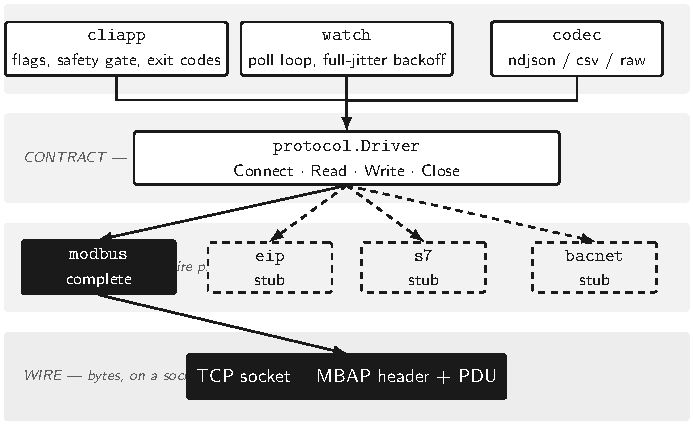
\includegraphics[width=0.95\linewidth]{architecture.pdf}
\caption{Layering. CLI concerns depend only on \code{protocol.Driver};
drivers are free to differ completely in how they parse an address
(a Modbus \code{table:address} string bears no resemblance to a CIP
symbolic tag or an S7 \code{DB.offset.bit} triple) as long as they
resolve to a \code{Value} on one side and wire bytes on the other.}
\label{fig:architecture}
\end{figure}

Two decisions in this boundary are worth stating explicitly because
each was a choice against a more ``obvious'' alternative.

\textbf{No shared address struct.} An earlier design considered a
single \code{Address\{Table, Offset, Type\}} struct used by every
driver. It was discarded: Modbus addresses a flat, four-table,
16-bit-register space; CIP addresses symbolic tags resolved through a
class/instance/attribute service request; S7comm addresses a
(DB-number, byte-offset, bit-offset, transport-size) tuple; BACnet
addresses an (object-type, instance, property) triple. A struct wide
enough to fit all four is a lowest-common-denominator that fits none
of them precisely, and would let a well-typed compile-time boundary
quietly hide the exact protocol-specific validation each address
grammar actually needs. \code{Driver.Read} and \code{Driver.Write}
instead take a plain \code{string}, and each driver owns its own
grammar and its own parser (\S\ref{sec:addressing}).

\textbf{No connection pooling.} \code{Driver} is single-connection,
single-endpoint, single-owner: one \otcat\ process talks to one
device over one socket. This mirrors how most real PLCs behave under
concurrent masters --- badly, in the common case of a single-threaded
protocol stack behind the Ethernet port --- and it keeps the client
free of a class of complexity (connection pool sizing, request
multiplexing, backpressure) that a CLI tool making tens of requests,
not tens of thousands, does not need. \S\ref{sec:mechanics} discusses
the consequence of this choice for the Modbus client specifically:
requests are serialized even though the wire protocol permits
pipelining.


\section{The Modbus Driver: Protocol Mechanics}
\label{sec:mechanics}

\subsection{Framing}

Every Modbus TCP Application Data Unit (ADU) is a 7-byte MBAP header ---
transaction identifier, protocol identifier (always zero), a length
field counting everything after itself, and a unit identifier ---
followed by a Protocol Data Unit (PDU) of at most 253
bytes~\cite{modbus_tcp_guide}. \otcat's client is deliberately
synchronous per connection (\S\ref{sec:driver-arch}): it writes one
full ADU, then blocks on \code{io.ReadFull} for exactly the response
length its own MBAP length field declares, rather than attempting to
demultiplex multiple in-flight transaction IDs. Figure~\ref{fig:sequence}
traces one successful transaction and the two failure modes every
caller of \code{Driver.Read} must handle: a protocol-level exception,
and a timeout with no response at all.

\begin{figure}[t]
\centering
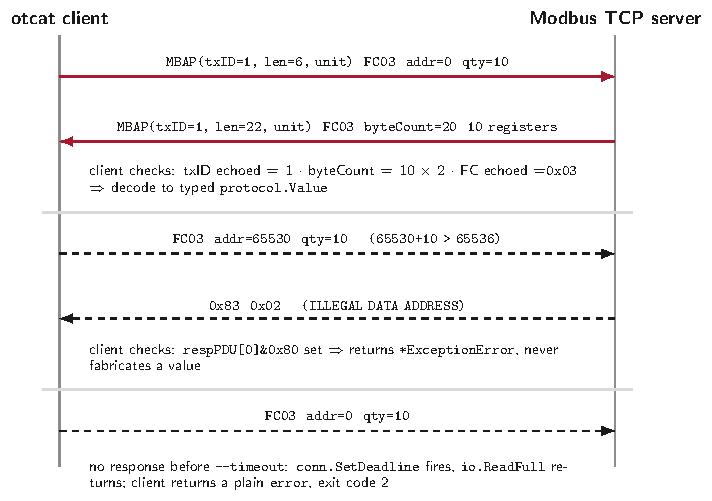
\includegraphics[width=0.95\linewidth]{sequence.pdf}
\caption{A read transaction, an exception response, and a timeout. The
client treats these as three distinct outcomes with three distinct
Go error shapes (\code{*ExceptionError} vs.\ a plain wrapped error),
which \S\ref{sec:verification} exploits to give scripts a stable exit
code per failure class.}
\label{fig:sequence}
\end{figure}

\subsection{The PDU Budget and Where the Protocol's Numbers Come From}

The Modbus specification states several apparently-arbitrary limits ---
125 registers per read, 2000 bits per read, 123 registers per write,
1968 bits per write --- without, in the specification text itself,
deriving them. They are in fact one constraint, applied four times:
the 253-byte PDU ceiling, minus each function's fixed header bytes,
divided by the size of one unit of payload. Figure~\ref{fig:pdubudget}
shows the derivation for the read-holding-registers case; \otcat's
client enforces all four limits client-side, before a byte reaches the
network, precisely because they are derivable and therefore checkable
without a round trip.

\begin{figure}[t]
\centering
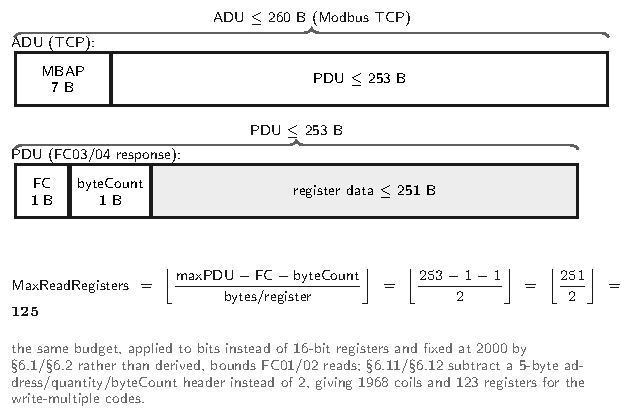
\includegraphics[width=0.95\linewidth]{pdu_budget.pdf}
\caption{The 253-byte PDU budget, and the arithmetic that turns it into
Modbus's four numeric limits. \code{internal/modbus/limits.go} states
each constant with this derivation as an inline comment rather than as
a bare literal.}
\label{fig:pdubudget}
\end{figure}

\subsection{Function Codes and Exception Taxonomy}

Table~\ref{tab:fc} lists the eight function codes \otcat\ implements ---
every data-access code the specification defines, and, by design,
nothing else (diagnostics, file-record access, and the FIFO/queue codes
are out of scope; they see negligible field use and each would import
its own address grammar for a feature otcat's audience rarely
needs). An exception response is distinguished by the high bit of the
echoed function code (Figure~\ref{fig:sequence}); \otcat\ decodes the
nine exception codes the specification defines into a typed
\code{ExceptionCode}, surfaced through a distinct Go error type
(\code{*ExceptionError}) rather than a generic error string, so that a
caller --- in particular, the CLI's exit-code logic --- can distinguish
``the device rejected this request'' from ``the network failed'' or
``the operator's input was malformed'' without string matching.

\begin{table}[t]
\centering
\caption{Function codes implemented. All eight are the complete
data-access subset of Modbus Application Protocol V1.1b3
\S6~\cite{modbus2012}.}
\label{tab:fc}
\small
\begin{tabular}{@{}L{0.9cm}L{2.5cm}L{2.6cm}@{}}
\toprule
\textbf{Code} & \textbf{Name} & \textbf{Table} \\
\midrule
0x01 & Read Coils & coil (bit, R/W) \\
0x02 & Read Discrete Inputs & discrete input (bit, R/O) \\
0x03 & Read Holding Registers & holding register (16-bit, R/W) \\
0x04 & Read Input Registers & input register (16-bit, R/O) \\
0x05 & Write Single Coil & coil \\
0x06 & Write Single Register & holding register \\
0x0F & Write Multiple Coils & coil \\
0x10 & Write Multiple Registers & holding register \\
\bottomrule
\end{tabular}
\end{table}



\section{Addressing Model}
\label{sec:addressing}

Modicon's original PLC documentation named four memory areas with a
five-digit reference number whose leading digit identifies the table:
\code{0}xxxx for coils, \code{1}xxxx for discrete inputs, \code{3}xxxx
for input registers, \code{4}xxxx for holding registers. The
convention predates the wire protocol's own 0-based, per-table
addressing by more than a decade and has outlived the company that
introduced it, yet it is still how every PLC vendor's documentation,
wiring diagram, and field engineer refers to a register --- which makes
it the one address format \otcat\ must accept even though it is not
what the wire protocol actually uses.

\otcat\ formalizes the translation as the deterministic function shown
in Figure~\ref{fig:addressing}: a numeral \(N\) given for table \(T\)
resolves to wire offset \(N - \mathrm{base}(T)\) if \(N\) falls inside
\(T\)'s classic five-digit band \([\mathrm{base}(T),\,
\mathrm{base}(T){+}9998]\), and to the literal offset \(N\) otherwise.
This is a real ambiguity, not a hypothetical one: a raw offset of, say,
\(42{,}000\) in the holding-register table is also a syntactically
valid classic reference number one past its band's start. \otcat\
resolves the ambiguity in the direction that matches every vendor
example (``holding register \code{40001}'' almost always means offset
zero, not offset \(40{,}001\)), and provides \code{--raw-address} as an
explicit, documented escape for the literal-offset case. The
alternative --- a heuristic threshold not tied to the convention's own
boundary --- would move the ambiguity to a threshold with no
documentation behind it at all; \otcat's rule has exactly one edge, and
it is the actual edge of the convention being reproduced.

\begin{figure}[t]
\centering
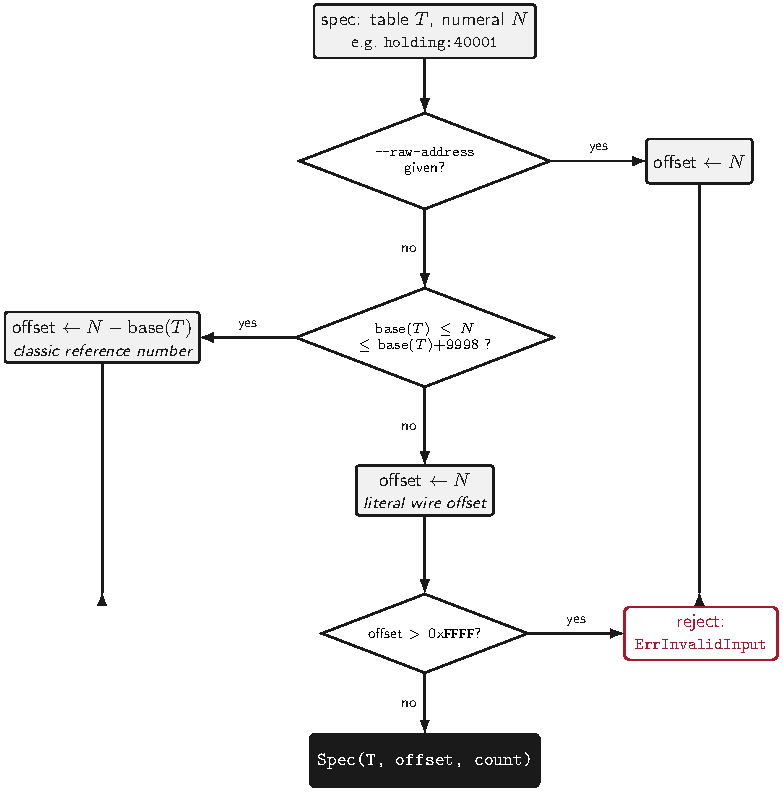
\includegraphics[width=0.92\linewidth]{address_resolution.pdf}
\caption{Address resolution. \code{ParseSpec} in
\code{internal/modbus/address.go}; property-tested for every table's
band boundary in \code{address\_test.go}.}
\label{fig:addressing}
\end{figure}

Coils are a further, easy-to-miss special case within this convention:
the leading-\code{0} table (\code{0}xxxx) is written without its
leading zero in every practical use --- ``coil 5,'' not ``coil
\code{00005}'' --- so \code{base(coil)} is \(1\), not \(0\); \otcat's
test suite pins this boundary explicitly
(\code{TestParseSpecClassicTranslation}) because it is exactly the kind
of off-by-one a generic ``subtract the leading digit's place value''
implementation gets wrong.

\section{Typed Register Codec}
\label{sec:codec}

A single Modbus register is 16 bits; every wider type --- 32-bit
integers and IEEE~754 \code{float32} in particular --- is a convention
layered on top of two consecutive registers, and the specification
fixes only one of the two axes that convention needs. \emph{Byte
order} within one register is fixed by the specification at big-endian
(high byte first)~\cite{modbus2012}, though \otcat\ still exposes it as
a client-side option because enough non-compliant field devices
byte-swap individual registers that assuming compliance is itself a
correctness risk. \emph{Word order} --- which of two consecutive
registers holds the more significant 16 bits --- is not specified at
all; vendors split roughly evenly between the two choices, and some
publish both as separate configuration options for the same device
family.

\otcat\ models this as two independent binary transformations,
\code{ByteOrder} \(\in\) \{big, little\} and \code{WordOrder} \(\in\)
\{high-first, low-first\}, composed by a single \code{Codec}:

\begin{lstlisting}[style=go]
type Codec struct {
    ByteOrder ByteOrder
    WordOrder WordOrder
}
func (c Codec) Decode(t DataType, regs []uint16)
    (interface{}, error)
func (c Codec) Encode(t DataType, literal string)
    ([]uint16, error)
\end{lstlisting}

The four combinations of the two axes are exactly the four register
orderings ("ABCD", "BADC", "CDAB", "DCBA") that industrial HMI/SCADA
configuration tools already name informally when asking an integrator
to pick a float encoding; \otcat\ names the two underlying axes instead
of the four combined labels, since the axes --- not the label --- are
what a datasheet actually specifies, and the four-letter names carry no
information a reader doesn't already get from ``byte order'' and ``word
order'' stated separately.

Correctness here is a round-trip property, not a fixed-example one: for
every \((\mathrm{ByteOrder}, \mathrm{WordOrder})\) pair and every
representable value of every supported type, \code{Decode(Encode(v))
= v}. \code{TestCodecRoundTripProperty} checks this directly --- 500
random samples of \code{uint16} and \code{int32} plus float32 samples
drawn from raw IEEE~754 bit patterns (so that subnormals, negative
zero, and NaN are exercised, not just ``typical'' values) across all
four \((\mathrm{ByteOrder}, \mathrm{WordOrder})\) combinations, 4{,}000
assertions per test run --- rather than the smaller set of fixed
worked examples (Table~\ref{tab:fc} and Figure~\ref{fig:pdubudget}'s
kind of example) that establish the mechanism is right for at least one
input.



\section{Concurrency, Polling, and Reliability}
\label{sec:reliability}

\subsection{The Write-Safety Gate}

\S\ref{sec:safety-philosophy} states the principle; Figure~\ref{fig:writesafety}
is its implementation as a state machine. Every path through it ends in
exactly one of two outcomes: the write is sent, or it is refused with
exit code 4 and a stated reason on stderr. There is no path that sends
a write silently. Three refusal cases are distinguished because each
has a different remedy: \code{--from-stdin} without \code{--confirm}
is refused because stdin is already consumed by the value stream, so no
confirmation prompt is even possible; a non-interactive caller (a cron
job, a CI step) without \code{--confirm} is refused for the same
structural reason; and an interactive caller who answers anything other
than \code{y}/\code{yes} is refused because that is what a
confirmation prompt is for.

\begin{figure}[t]
\centering
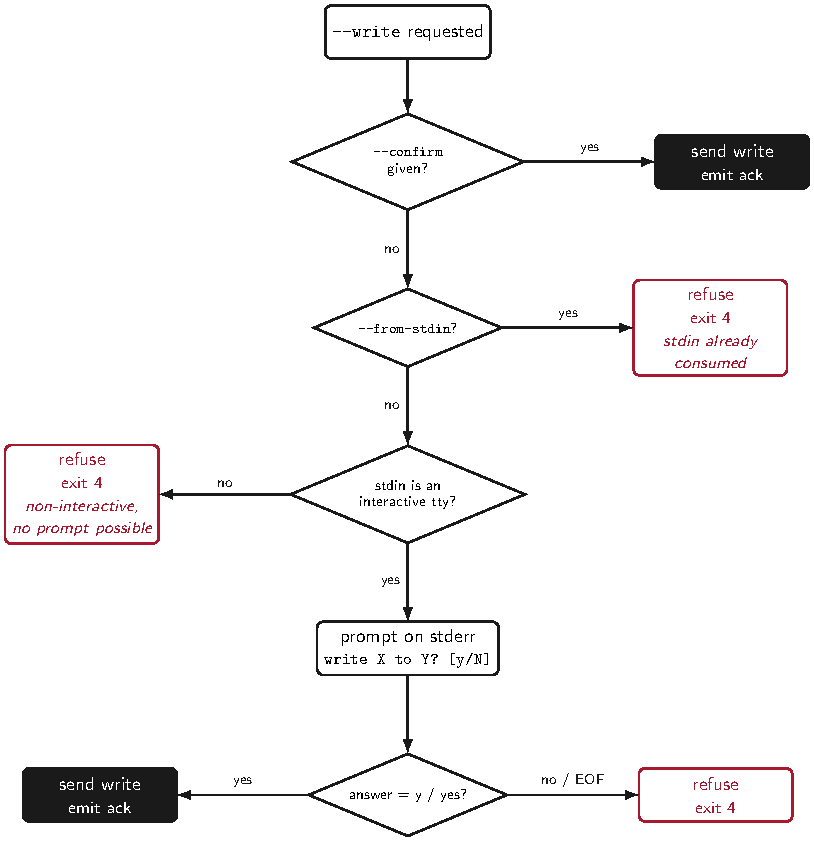
\includegraphics[width=0.92\linewidth]{write_safety.pdf}
\caption{The write-safety gate. \code{gateWrite} in
\code{internal/cliapp/actions.go}; every terminal state is reachable
and covered by \code{cliapp\_test.go} (\S\ref{sec:verification}).}
\label{fig:writesafety}
\end{figure}

\code{--dry-run} sits outside this gate entirely, by construction
rather than by an additional check: the CLI's dispatch computes the
dry-run \code{WritePlan} and returns before \code{Driver.Connect} is
ever called (\code{cliapp.go}, \code{Run}), so a dry run cannot reach
the network even if every other check in the codebase were removed.
\code{ExplainWrite} and \code{Write} share one internal encoding
routine precisely so that what a dry run reports and what an actual
write sends cannot drift apart --- they are, structurally, the same
computation, with I/O attached in one case and not the other
(\code{TestDriverExplainWriteMatchesWrite} asserts this directly by
comparing a planned write's registers against the registers an actual
write, to the same address and literal, produces on the wire).

\subsection{Polling and Backoff}

\code{--watch} polls at a fixed \code{--interval} while reads succeed.
On failure, retrying at the same interval has two costs: it can
overwhelm a device that is mid-recovery from whatever caused the
failure, and, with more than one client polling the same segment, it
synchronizes every client's retries into a periodic burst rather than
spreading them out. \otcat\ instead uses \emph{Full Jitter} exponential
backoff~\cite{brooker2015}:
\[
\mathrm{delay}(a) = \mathrm{Uniform}\bigl(0,\ \min(\mathrm{max}, \ \mathrm{base} \cdot 2^{a-1})\bigr)
\]
for failure count \(a \ge 1\), resetting to \(a{=}0\) after every
successful read. This is chosen deliberately over two more obvious
alternatives: plain exponential backoff with no randomness still
perfectly synchronizes every client that failed at the same instant
(it reduces load but not correlation between clients), and ``Equal
Jitter'' (\(\mathrm{delay} = \mathrm{ceiling}/2 + \mathrm{Uniform}(0,
\mathrm{ceiling}/2)\)) never lets the delay approach zero, wasting the
fast-recovery case where a device is back within milliseconds. Full
Jitter's own analysis shows it minimizes total client-side retry
volume for a given amount of collision avoidance among the
three~\cite{brooker2015}; Algorithm~\ref{alg:poll} gives the full loop.

\begin{algorithm}[t]
\caption{\code{watch.Run} polling loop}
\label{alg:poll}
\begin{algorithmic}[1]
\State $a \gets 0$ \Comment{consecutive failure count}
\While{context not cancelled}
  \State $v, err \gets \Call{Read}{}$
  \If{$err \neq \mathrm{nil}$}
    \State $a \gets a + 1$
    \State $\mathrm{sleep}\bigl(\mathrm{Uniform}(0, \min(\mathrm{maxBackoff}, \mathrm{interval} \cdot 2^{a-1})) \bigr)$
    \State \textbf{continue}
  \EndIf
  \State $a \gets 0$
  \State \Call{Emit}{$v$} \Comment{one ndjson line, flushed}
  \If{count limit reached}\ \textbf{return}\ \EndIf
  \State $\mathrm{sleep}(\mathrm{interval})$
\EndWhile
\end{algorithmic}
\end{algorithm}



\section{Verification Methodology}
\label{sec:verification}

\otcat's test suite combines four complementary techniques, each aimed
at a different class of defect a protocol implementation is prone to.

\textbf{Unit tests} pin exact wire encodings against the
specification's own worked examples --- Table~\ref{tab:fc}'s FC~0x01
example (\code{0xCD, 0x01} decoding to a specific 10-bit pattern) is
taken directly from Modbus Application Protocol V1.1b3 \S6.1, not
constructed independently, so a passing test is evidence against the
specification text itself, not merely against the implementation's own
prior behavior.

\textbf{Property-based round-trip tests} (\S\ref{sec:codec}) check a
relationship that must hold for \emph{every} input in a large random
sample, rather than for a curated few, and are the only technique in
the suite that caught an entire class of the codec's behavior (word
order composed with byte order across all four combinations) that a
reasonable set of hand-picked examples could plausibly have missed.

\textbf{Integration tests} run the real client against a real,
spec-correct mock Modbus TCP server (\code{internal/mock}) over an
actual TCP socket on loopback --- not a mocked transport --- including
fault injection (\code{WithLatency}, \code{WithDropRate}) to exercise
timeout and mid-transaction disconnection paths that are otherwise hard
to trigger deterministically.

\textbf{Coverage-guided fuzzing} targets every function that parses
bytes or text this project does not control: the MBAP header decoder,
the two response-body decoders, the address-spec parser, and the
write-literal encoder. Five fuzz targets ran a combined 65 CPU-seconds
in this paper's evaluation environment with zero crashes; \code{go
vet}, \code{gofmt}, and the race detector (\code{go test -race}) are
clean across the entire tree, and CI (\S\ref{sec:evaluation}) runs a
10-second-per-target fuzz pass on every commit as a cheap regression
net rather than a one-time audit.

\subsection{Case Study: A Bug the Test Suite Found}

One instance is worth reporting in detail because it is evidence for
the methodology, not just a bullet point about it. An end-to-end CLI
test asserted that a malformed address spec (\code{bogus:0}, an
unknown table name supplied to \code{--read}) should produce a usage
error --- exit code~1 --- since it is an operator mistake, not a device
or network failure. The test failed: the actual exit code was~5 (I/O
error), because the address parser's error was a plain, unwrapped
\code{fmt.Errorf} that the CLI's error classifier could not distinguish
from a genuine output-encoding failure. The fix introduces a sentinel,
\code{modbus.ErrInvalidInput}, wrapped (via \code{\%w}) into every
malformed-input error path across the address parser, the type/order
parsers, and the write-literal encoder, and taught the CLI's classifier
to check for it with \code{errors.Is}. The mechanism generalizes: any
future malformed-input error in the Modbus driver is now
correctly classified without a case-by-case fix, provided it is
produced through the same wrapping convention. This is included here
specifically because a paper claiming a rigorous test methodology
should show the methodology catching something, not merely assert that
it would.



\section{Evaluation}
\label{sec:evaluation}

\subsection{Methodology and Its Honest Limits}

Every number in this section comes from \code{benchmarks/} in the
accompanying repository, produced by the exact commands in
\code{benchmarks/README.md} and reproduced by any checkout: \code{go
test -bench=. -benchmem}, three iterations per benchmark, arithmetic
mean reported; the latency distribution comes from
\code{otcat-latencyprobe}, a companion tool built specifically to
measure percentiles (not just means) rather than from the Go
benchmarking harness alone. All full round-trip measurements are over
TCP loopback (\code{127.0.0.1}) on a single-core sandbox VM.

This needs one honest caveat, stated plainly rather than buried:
loopback measures \otcat's \emph{own} encode/dispatch/decode overhead
with real network latency approximately zeroed out. It is a ceiling on
achievable throughput against an infinitely fast device, not a
prediction of performance against a real PLC on a real LAN, where
request/response latency is normally dominated by the device's own
response time --- commonly single-digit to tens of milliseconds for a
serial-backed TCP gateway, three orders of magnitude larger than
anything measured here --- rather than by \otcat.

\subsection{Pure Computational Cost}

Figure~\ref{fig:opcosts} breaks down the CPU cost of each stage with no
I/O involved. Encoding a read request is sub-nanosecond (it is five
bytes written into a pre-sized slice); decoding a ten-register response
and parsing a classic address spec are both under 100~ns; ndjson
encoding, at roughly 900~ns, is the single largest fixed cost in the
pipeline and is dominated by \code{encoding/json}'s reflection-based
marshaling of the output struct --- a cost paid once per emitted value,
independent of read width.

\begin{figure}[t]
\centering
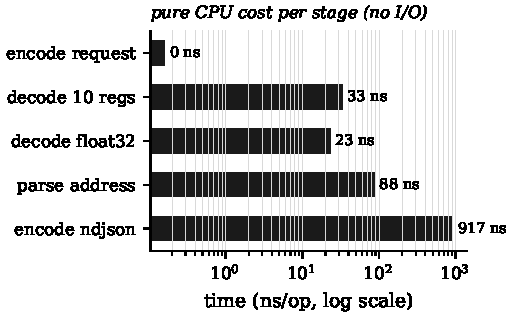
\includegraphics[width=0.95\linewidth]{op_costs.pdf}
\caption{Per-stage CPU cost, no I/O (Table~\ref{tab:bench} gives exact figures).}
\label{fig:opcosts}
\end{figure}

\subsection{Round-Trip Latency and Throughput}

Figure~\ref{fig:latency} is the distribution behind
Table~\ref{tab:bench}'s single mean figure for a 10-register read:
10{,}000 sequential requests over one persistent connection, median
5~\textmu s, p99 26~\textmu s, p99.9 47~\textmu s. The right tail (max
579~\textmu s across 10{,}000 samples) is consistent with occasional Go
garbage-collector pauses and OS scheduling jitter on a single-core VM,
not with anything read-width- or protocol-dependent --- it appears
identically in the 1-register and 125-register cases.

\begin{figure}[t]
\centering
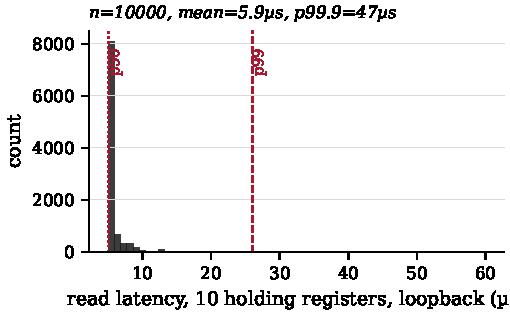
\includegraphics[width=0.95\linewidth]{latency_hist.pdf}
\caption{Read latency distribution, $n=10{,}000$, loopback.}
\label{fig:latency}
\end{figure}

Figure~\ref{fig:throughput} shows measured throughput falling gently as
read width grows from 1 to 125 registers per request --- 155{,}304 to
135{,}919 reads/sec, a 12.5\% decrease across a 125$\times$ increase in
payload size --- which is the expected shape for a client whose fixed
per-request overhead (one syscall round trip, one MBAP header, one
ndjson encode) dominates over its marginal per-byte decode cost.

\begin{figure}[t]
\centering
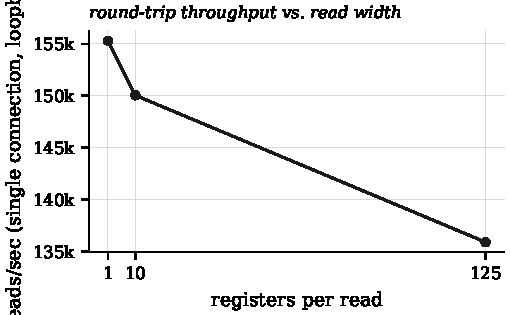
\includegraphics[width=0.95\linewidth]{throughput.pdf}
\caption{Round-trip throughput vs.\ registers per read, single
connection, loopback.}
\label{fig:throughput}
\end{figure}

\begin{table}[t]
\centering
\caption{Selected benchmark results (mean of 3 runs). Full results in \code{benchmarks/raw\_results.txt}.}
\label{tab:bench}
\small
\begin{tabular}{@{}L{4.0cm}rrr@{}}
\toprule
\textbf{Benchmark} & \textbf{ns/op} & \textbf{B/op} & \textbf{allocs} \\
\midrule
Encode read request & 0.16 & 0 & 0 \\
Decode 10-register response & 33.2 & 24 & 1 \\
Decode float32 (codec) & 23.1 & 8 & 2 \\
Parse classic address spec & 87.9 & 48 & 1 \\
Encode ndjson output & 917.2 & 168 & 3 \\
Full jitter backoff draw & 7.8 & 0 & 0 \\
\midrule
Round trip, 1 register & 6{,}439 & 80 & 10 \\
Round trip, 10 registers & 6{,}665 & 160 & 10 \\
Round trip, 125 registers & 7{,}357 & 1{,}112 & 10 \\
Round trip, single-register write & 6{,}431 & 88 & 10 \\
Driver.Read end-to-end (parse+I/O+decode) & 7{,}025 & 160 & 14 \\
\bottomrule
\end{tabular}
\end{table}

The allocation count is flat at 10 per round trip regardless of read
width (Table~\ref{tab:bench}): \otcat's client allocates for the
request buffer, the response header buffer, and the response body
buffer once each, not per register, which is why bytes-per-op scales
with read width while allocs-per-op does not.

\subsection{Cross-Implementation Interoperability}
\label{sec:interop}

Every result above validates \otcat\ against \code{internal/mock}, a
server this project wrote itself --- necessary for controlled fault
injection (\S\ref{sec:verification}), but structurally unable to catch
a specification misreading shared by both the client and the mock.
The closest available substitute for physical-device testing is
agreement with servers neither authored by, nor written for, this
project: pymodbus~\cite{pymodbus} (Python) and
modbus-serial~\cite{modbus_serial_npm} (JavaScript), two independently
maintained, widely deployed open-source Modbus stacks. Both were run
unmodified; \otcat's client was pointed at each in turn and exercised
across every function code in Table~\ref{tab:fc} --- reads and writes,
scalar and array, all four tables, and (against pymodbus) a
genuine out-of-range read that the \emph{server}, not \otcat, rejected,
correctly decoded as \code{ExIllegalDataAddress} and mapped to exit
code 3. All results matched expectation with zero discrepancies
between the two independent servers and \otcat's own mock. Full
commands and captured output are in
\code{docs/interop\_testing.md}, reproducible with the two scripts in
\code{scripts/}.

This raises confidence beyond self-testing without closing the gap
\S\ref{sec:limitations} already names: independently-implemented
\emph{software} stacks tend to converge on strict specification
compliance, which is exactly the property field firmware is least
guaranteed to share. Table~\ref{tab:interop} summarizes what was, and
was not, exercised by this method.

\begin{table}[t]
\centering
\caption{Cross-implementation interoperability coverage.}
\label{tab:interop}
\small
\begin{tabular}{@{}L{2.6cm}L{2.6cm}L{2.5cm}@{}}
\toprule
& \textbf{pymodbus} & \textbf{modbus-serial} \\
\midrule
FC 01/02/03/04 (read) & \checkmark & \checkmark \\
FC 05/06 (write single) & \checkmark & \checkmark \\
FC 16 (write multiple) & \checkmark & --- \\
Server-issued exception & \checkmark & --- \\
32-bit float, word order & \checkmark & \checkmark \\
\bottomrule
\end{tabular}
\end{table}



\section{Case Study: A Closed-Loop Demonstration}
\label{sec:case-study}

The figures above measure otcat in isolation. This section closes the
loop: a physically-modeled process, driving a real Modbus TCP server
(\code{otcat-mockplc}), observed end to end by an unmodified \otcat\
binary --- the same one a reader would build from this repository ---
through an actual TCP socket. Every number and every point on
Figure~\ref{fig:tank} is output the tool itself produced; nothing in
this section is a mock-up of what the output would look like.

\subsection{The Process}

\code{internal/mock.TankProcess} simulates one level-controlled tank: a
PI controller driving an inlet valve against gravity-fed outflow
through a fixed orifice, integrated with forward Euler at a fixed
100~ms step. Outflow follows Torricelli's law; net level change
integrates flow over the tank's cross-section \(A\):
\begin{align}
\frac{dh}{dt} &= \frac{Q_{in}(t) - Q_{out}(t)}{A} \\
Q_{out}(t) &= k' \sqrt{\max(h, 0)} \\
Q_{in}(t) &= \mathrm{valve}(t) \cdot Q_{max} \\
\mathrm{valve}(t) &= \mathrm{clamp}\bigl(K_p e + K_i \!\!\int\!\! e\, dt,\ 0,\ 1\bigr) \\
e(t) &= h_{setpoint} - h(t)
\end{align}
with \(k'\) folding the discharge coefficient and \(\sqrt{2g}\)
together. The controller writes its output as a fixed-point percentage
(two implied decimal places in a plain \code{uint16}, e.g.\ \(1523 =
15.23\%\)) into holding register~0 --- the same encoding a real PLC
commonly uses to carry a fractional analog value without a native
float type, chosen here so the demonstration exercises an encoding
choice a real deployment would actually make, not merely one convenient
for this paper.

\subsection{Observation}

\begin{lstlisting}[style=sh]
otcat-mockplc --addr 127.0.0.1:15021 &
otcat --modbus 127.0.0.1:15021 \
  --watch holding:0 --raw-address \
  --interval 100ms --count 300 --json \
  > tank_watch.ndjson
\end{lstlisting}

300 samples, 100~ms apart, 30 seconds of wall-clock time, one ndjson
line per sample, each independently valid JSON:

\begin{lstlisting}[style=sh, basicstyle=\ttfamily\scriptsize]
{"address":"holding:0","type":"uint16",
 "value":2023,"quality":"good",
 "ts":"2026-07-19T13:38:16.147Z","raw":[2023]}
\end{lstlisting}

Figure~\ref{fig:tank} plots \code{value}$/100$ against elapsed time
directly from this file. The level rises from its 20.23\% initial
condition toward the 60\% setpoint with the smooth, non-oscillatory
approach a critically-damped-ish PI loop on a square-root nonlinearity
produces --- the process model's own dynamics, not anything otcat adds
or smooths; \otcat\ reports exactly the integer the server held at each
poll instant.

\begin{figure}[t]
\centering
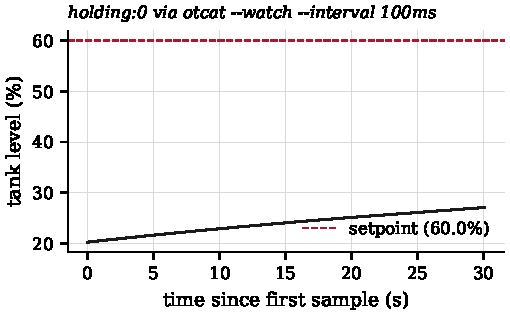
\includegraphics[width=0.95\linewidth]{tank_watch.pdf}
\caption{holding:0, read via \code{otcat --watch --interval 100ms},
300 consecutive samples, plotted directly from the tool's own ndjson
output.}
\label{fig:tank}
\end{figure}



\section{Limitations, Threat Model, and Roadmap}
\label{sec:limitations}

\subsection{What the Write-Safety Gate Is Not}

Figure~\ref{fig:writesafety}'s gate prevents an operator's own accident
--- a mistyped address, a re-run script, a copy-paste error --- from
reaching a device silently. It is not an authentication mechanism, and
Modbus TCP gives it no cryptographic material to build one from: any
process that can open a TCP connection to a device's Modbus port can
issue any write that device accepts, \otcat\ or not. A threat model
that includes an adversary already on the OT network segment is out of
scope for what a protocol client, running locally, can meaningfully
defend against; that boundary belongs to network segmentation
(\S\ref{sec:related-work}'s Purdue Model reference) and to the OT
security monitoring layer \otcat\ deliberately does not attempt to be.

\subsection{Protocol Coverage}

Three drivers are registered in the CLI's \code{--help} output and
fail immediately with a clear error rather than attempting their wire
protocol. What each would require, concretely:

\begin{itemize}
\item \textbf{EtherNet/IP (CIP).} A Register/UnRegister Session
encapsulation handshake; Unconnected Send (service~0x52) and Forward
Open/Close for connected messaging; \code{Get\_Attribute\_Single}/
\code{Get\_Attribute\_List} CIP services; symbolic tag-name segment
encoding; and vendor-specific structured-tag (Rockwell UDT) layout
handling, since CIP does not fully standardize UDT wire serialization.
\item \textbf{S7comm.} COTP (RFC~1006) connection setup carrying an S7
PDU negotiation, then item addresses encoded as (area, DB number, byte
offset, bit offset, transport size) tuples. Siemens has not published
this protocol; every existing open implementation is derived from
packet capture rather than a specification --- exactly the provenance
this project is unwilling to ship a write path on top of without
independent cross-validation.
\item \textbf{BACnet/IP.} UDP-native, requiring Who-Is/I-Am discovery
before an address is resolvable, with APDUs built from a
tag-length-value encoding materially larger in scope than Modbus's
fixed-position PDU.
\end{itemize}

Each future driver is held to the bar Modbus was built to here: a
from-specification (or, absent one, cross-validated) codec; a mock
server exercising every service it claims; fuzz coverage on every
network-facing parser; and, for any write path, a dry-run mode. A
driver that cannot clear that bar stays a stub.

\subsection{Transport and Concurrency}

Modbus RTU/ASCII (serial) transport is not implemented; \otcat\ speaks
Modbus TCP only. \S\ref{sec:driver-arch}'s single-connection,
non-pipelined client trades away throughput the wire protocol would
technically permit (multiple in-flight transactions per connection)
for immunity to the single-threaded-gateway failure mode that
trade avoids; \S\ref{sec:evaluation}'s throughput figures should be
read as ``per connection,'' not as a ceiling on what a differently
architected client could achieve against a device that actually
supports pipelining.

\subsection{Language Bindings}

A Python package (\code{python/}, distributed separately from the Go
module) extends \otcat's reach into pandas-based data science,
FastAPI/WebSocket services, threshold-based alerting, and read-only OT
asset-discovery workflows. It is deliberately a subprocess wrapper
around the same compiled Go binary described throughout this paper,
not a reimplementation of the protocol in Python: every read and write
issued through it still passes through the identical, tested Modbus
client, at the cost of one process spawn per call (negligible next to
a Modbus round trip; see Table~\ref{tab:bench}). Its one deliberate
deviation from the Go CLI is documented, not accidental: library calls
default to treating a write as already-decided by the calling code
(\code{confirm=True}), the opposite of the CLI's human-facing default,
since a keystroke-typo is not a failure mode a function call can have.
The read-only auditing module carries forward \S\ref{sec:limitations}'s
threat-model boundary verbatim: it enumerates and fingerprints, it
never writes, and it is not an authorization bypass for equipment one
is not already permitted to test.

\section{Conclusion}

\otcat\ is a small tool built on a large premise: that the property
which made \code{netcat} indispensable was never protocol-agnosticism
for its own sake, but the discipline of putting exactly one
self-describing unit of information on stdout and taking exactly one
back from stdin, so that everything else --- filtering, alerting,
historians, ad hoc curiosity --- could be somebody else's problem, solved
with tools that already exist. Operational technology's protocols are
too structured for \code{netcat}'s own protocol-blindness to transfer
directly; \otcat's contribution is showing that the discipline
transfers even when the blindness cannot --- that a Modbus client can be
complete, formally addressed, round-trip-tested, fuzzed, and
transparent about exactly what it will send before it sends it, while
still being one flag away from a Unix pipe. The three protocols left
as honest stubs are not an admission that this was out of reach; they
are this paper's clearest statement of what ``complete'' is worth
holding out for.


\appendices

\section{Command-Line Reference}

\begin{lstlisting}[style=sh, basicstyle=\ttfamily\scriptsize]
otcat --modbus HOST:PORT --read TABLE:ADDR[:COUNT] [flags]
otcat --modbus HOST:PORT --watch TABLE:ADDR[:COUNT] [flags]
otcat --modbus HOST:PORT --write TABLE:ADDR \
      --value LITERAL --confirm [flags]
cat values.txt | otcat --modbus HOST:PORT \
      --write TABLE:ADDR --from-stdin --confirm
\end{lstlisting}

\noindent \code{otc} is installable and behaves identically to
\code{otcat} in every example above and throughout this paper.

\noindent Address grammar, in EBNF:
\begin{lstlisting}[style=sh, basicstyle=\ttfamily\scriptsize]
spec    = table ":" address [ ":" count ] ;
table   = "coil" | "discrete" | "holding" | "input" ;
address = digit , { digit } ;
count   = digit , { digit } ;
\end{lstlisting}

\begin{table}[h]
\centering
\caption{Exit codes.}
\label{tab:exit}
\small
\begin{tabular}{@{}rL{6.6cm}@{}}
\toprule
\textbf{Code} & \textbf{Meaning} \\
\midrule
0 & success \\
1 & usage error --- bad flags, malformed spec, bad literal \\
2 & connection error --- dial/timeout/refused \\
3 & protocol error --- device returned a Modbus exception \\
4 & write aborted --- not confirmed \\
5 & I/O error --- e.g.\ broken output pipe \\
130 & \code{--watch} stopped cleanly by SIGINT/SIGTERM \\
\bottomrule
\end{tabular}
\end{table}

\begin{thebibliography}{99}

\bibitem{mcilroy1978}
M.~D. McIlroy, E.~N. Pinson, and B.~A. Tague, ``UNIX time-sharing
system: Foreword,'' \emph{The Bell System Technical Journal}, vol.~57,
no.~6, part~2, pp.~1899--1904, 1978.

\bibitem{nc_manpage}
OpenBSD Project, ``nc(1) --- OpenBSD manual pages,'' netcat originally
released by \emph{Hobbit}, 1995. [Online]. Available:
\url{https://man.openbsd.org/nc.1}

\bibitem{modbus2012}
Modbus Organization, ``MODBUS Application Protocol Specification
V1.1b3,'' Apr. 26, 2012. [Online]. Available:
\url{https://www.modbus.org/docs/Modbus_Application_Protocol_V1_1b3.pdf}

\bibitem{modbus_tcp_guide}
Modbus-IDA, ``MODBUS Messaging on TCP/IP Implementation Guide V1.0b,''
Oct. 24, 2006. [Online]. Available:
\url{https://www.modbus.org/docs/Modbus_Messaging_Implementation_Guide_V1_0b.pdf}

\bibitem{brooker2015}
M.~Brooker, ``Exponential backoff and jitter,'' \emph{AWS Architecture
Blog}, Mar. 2015. [Online]. Available:
\url{https://aws.amazon.com/blogs/architecture/exponential-backoff-and-jitter/}

\bibitem{williams1994}
T.~J. Williams, ``The Purdue enterprise reference architecture,''
\emph{Computers in Industry}, vol.~24, no.~2--3, pp.~141--158, 1994.

\bibitem{fireeye_triton2017}
FireEye/Mandiant Threat Research, ``Attackers deploy new ICS attack
framework `TRITON' and cause operational disruption to critical
infrastructure,'' Dec. 2017. [Online]. Available:
\url{https://www.fireeye.com/blog/threat-research/2017/12/attackers-deploy-new-ics-attack-framework-triton.html}

\bibitem{odva_cip}
ODVA, Inc., \emph{The CIP Networks Library, Volume 2: EtherNet/IP
Adaptation of CIP}. Ann Arbor, MI: ODVA.

\bibitem{ashrae135}
ASHRAE/ANSI Standard 135, \emph{BACnet --- A Data Communication
Protocol for Building Automation and Control Networks}. Atlanta, GA:
ASHRAE.

\bibitem{rashid2025modbus}
M.~Rashid \emph{et~al.}, ``Methodology for assessing existing
vulnerabilities in industrial control systems,'' \emph{Procedia
Computer Science}, vol.~259, pp.~1983--1993, 2025.

\bibitem{pymodbus}
pymodbus contributors, ``pymodbus: A full Modbus protocol implementation
in Python,'' open-source software. [Online]. Available:
\url{https://pypi.org/project/pymodbus/}

\bibitem{libmodbus}
S.~Santos, ``libmodbus: A Modbus library for Linux, Mac OS, FreeBSD,
QNX and Windows,'' open-source software. [Online]. Available:
\url{https://libmodbus.org/}

\bibitem{mbpoll}
\emph{mbpoll}, a command-line Modbus master utility for RTU/ASCII/TCP,
open-source software, distributed via major Linux package repositories
and \url{https://github.com/}.

\bibitem{modbus_serial_npm}
\emph{modbus-serial} contributors, ``modbus-serial: A pure JavaScript
Modbus RTU/TCP implementation for Node.js,'' open-source software.
[Online]. Available: \url{https://www.npmjs.com/package/modbus-serial}

\end{thebibliography}

\end{document}
